\usetikzlibrary{automata, arrows, shapes, patterns}

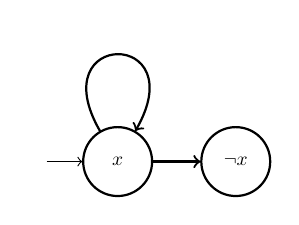
\begin{tikzpicture}
    \tikzstyle{n}=[state,circle,scale=0.7,thick, minimum size=1.25cm]
    \tikzstyle{e}=[->,thick]

    \def\dx{1.5}

    \node[initial, initial text={}, n] (A) at (0,0) {$x$};
    \node[n] (B) at (\dx cm, 0cm) {$\neg x$};

    \path[e] (A) edge [out=120,in=60,distance=1.5cm] (A);
    \draw[e] (A) -- (B);

\end{tikzpicture}
